\Block{A Problem with POCL Planning}{
\begin{itemize}
    \item What is POCL planning?
    \begin{itemize}
  	    \item It is a planning technique which searches the space of partially ordered sets of actions, called partial plans, rather than the space of states.
  	    \item Causal links are used to represent the causal relationships between actions, linking an effect of a producer action to a precondition of a consumer action.
  	    \item Any action which deletes a precondition being protected by a causal link will be ordered before the producer action or after the consumer action. 
    \end{itemize}
    \item What are the benefits of POCL planning?
    \begin{itemize}
  	    \item Since actions are only partially ordered, a single partial plan can represent up to a factorial number of action sequences.
  	    \item Causal links also hold a great deal of information about the search space and how it can be navigated.
    \end{itemize}
    \item POCL planners currently underperform classical state-based planners, so what's the issue?
    \begin{itemize}
  	    \item The information density of partial plans, while allowing for much more compact search, also make it difficult to create informed heuristics, which are vital for efficiently exploring the search space.
  	    \item Current POCL heuristics run efficiently by ignoring large amounts of information with the partial plans they are calculated on, but this wastes the effort spent on finding this information, and negates many of the advantages of POCL planning.
    \end{itemize}
\end{itemize}
}
Figure 1 shows the information completely ignored by the additive heuristic, a state of the art POCL heuristic, in red.\\
% insert a figure for imgs/plan-1.png
\begin{figure}[ht]
  \centering
  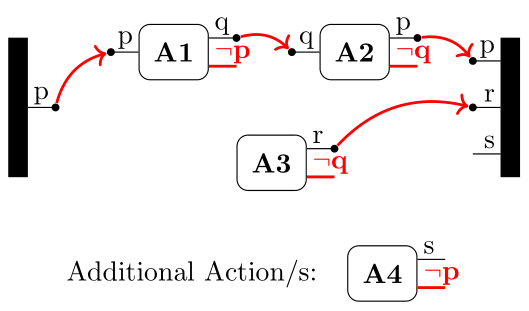
\includegraphics[width=0.8\textwidth]{imgs/plan-1.png}
  \caption{An example partial POCL plan, with the information ignored by the additive heuristic in red.}
\end{figure}

\Block{A Potential Solution: NP-Hard Heuristics}{
\begin{itemize}
    \item How do we make POCL heuristics more informed?
	\begin{itemize}
		\item Relaxations which lead to polytime problems in state-based search are often NP-hard in POCL planning.
		\item But why is an NP-hard heuristic inherently bad? It is possible that the benefits could outweigh the costs.
		\item Since a POCL plan can represent a factorial number of action sequences, informed search could significantly reduce the search space, which is particularly promising for detecting infeasible problems early.
	\end{itemize}
	\item Delete-relaxation allows for a potential NP-complete heuristic for POCL planning. 
	\begin{itemize}
		\item Delete-relaxation is a common problem relaxation used for heuristics in state-based planning, and involves solving the plan with all delete effects of future actions removed.
		\item Due to the need to consider the orderings and causal links of the actions already within the partial plan, which remain unrelaxed, this relaxed problem class is NP-Complete for POCL planning.
		\item We implement and evaluate this delete-relaxation heuristic in our report.
	\end{itemize}
\end{itemize}
}

Figure 2 shows what information is relaxed in the delete-relaxation heuristic we propose, note that additional actions still respect causal links, and hence their delete effects are relaxed but not completely ignored.\\
% insert a figure for imgs/plan-2.png
\begin{figure}[ht]
  \centering
  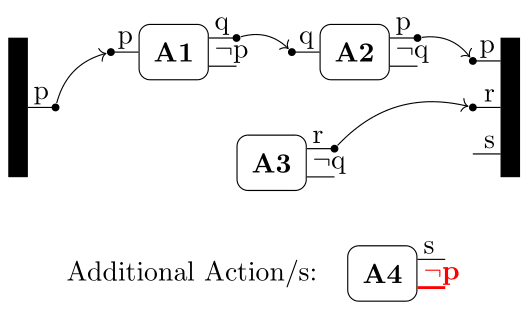
\includegraphics[width=0.8\textwidth]{imgs/plan-2.png}
  \caption{An example partial POCL plan, with the information relaxed by our heuristic in red.}
\end{figure}


\Block{An Integer Linear Programming Model}{
\begin{itemize}
    \item We use an Integer Linear Program (ILP) model to represent delete-relaxed POCL problems, and act as our heuristic.
	\begin{itemize}
	    \item Actions and propositions are associated with time variables, which are constrainted to enforce preconditions and effects.
		\item Causal links are compiled away before delete-relaxation occurs, allowing for the relaxed problem to be solved with causal links still being respected.
		\item Delete effects of actions already within the partial plan, and hence not delete-relaxed, create additional proposition and action variables to account for the potential need to re-establish deleted propositions.
		\item Ordering constraints can be directly translated into the ILP.
	\end{itemize}
\end{itemize}
}


\Block{Summary of Results}{
\begin{itemize}
    \item While our heuristic leads to slower solving times for both feasible and infeasible problems, the heuristic is significantly more informed than all other heuristics tested. This suggests that improvements to efficiency could lead to this heuristic being viable. Figure 3 shows the number of expanded nodes for our heuristic compared to the additive heuristic.
\end{itemize}
}

\begin{figure}[ht]
\centering
\begin{tikzpicture}
\begin{axis}[
	%title={Number of Generated Search Nodes (Log Scale)},
	xlabel style={anchor=north,yshift=-1em},  % Move x-axis label down
	ylabel style={anchor=east,yshift=1.5em,xshift=4.5em},   % Move y-axis label to the left
	xlabel={Delete-Relaxation Heuristic},
	ylabel={Additive Heuristic},
	scale only axis,
	height=15cm,
	width=15cm,
	xmode=log,
    ymode=log,
    xmin=1,
    xmax=1000000,
    ymin=1,
    ymax=1000000
]
\addplot+[
	mark=*,
	mark size=3pt,
	color=black,
	only marks]
table[]
{data/test.dat};
\addplot[black] coordinates {(1,1) (1000000,1000000)};
\end{axis}
\end{tikzpicture}
\caption{A Comparison of the number of search nodes generated by our delete-relaxed heuristic and the additive heuristic for problems from the 3rd International Planning Competition.}
\end{figure}